\chapter{Material und Methoden}

Dieses Kapitel stellt die Deep-Learning-Architektur und das Dataset genauer vor, mit dem sich diese Thesis beschäftigt.
Grundlage der \glspl{can} sind die \glspl{gan}, weshalb diese zuerst betrachtet werden.
Anschließend erfolgt eine Erläuterung zur Architektur der \glspl{can} und welche Besonderheiten in Bezug auf die Segmentierung auftreten.
Zum Schluss wird das Datenmaterial vorgestellt, das in dieser Arbeit zum Einsatz kommt.



\section{Generative Adversarial Networks}

Maschinelles Lernen hat eine Klasse Algorithmen hervorgebracht, die sehr viele gelabelte Daten benötigen.
Um die Menge an benötigten Daten zu verringern, wird im Deep-Learning-Bereich an Ansätzen geforscht, die neue Trainingssamples generieren, fehlende Werte ausfüllen oder durch unüberwachtes Lernen oder Transfer Learning zu einer Verbesserung beitragen können~\cite{Goodfellow.2016}.
Viele dieser Entwicklungen basieren auf Modellen, die Wahrscheinlichkeitsverteilungen über die Trainingsdaten abschätzen, und solche Abschätzungen sind nur durchführbar, wenn man Inferenz approximiert.

Eine solche approximierte Inferenz bedingt eine Normalisierung über eine Konstante, deren Berechnung wiederum nur durch Approximation durchführbar wird.
Viele dieser Approximationen werden wegen der Abhängigkeit von allen Modellparametern mit wachsender Dimensionalität exponentiell schwieriger zu berechnen.
Häufig werden auf Markov-Ketten basierende Monte-Carlo-Methoden~\cite{Koller.2009} zur Berechnung der Normalisierungskonstante genutzt, aber diese funktionieren meist nur bei Konstellationen mit wenigen, nicht klar separierten Moden der Wahrscheinlichkeitsverteilung~\cite{Goodfellow.2016}.

Die \glspl{gan} von \citeauthor{Goodfellow.2014}~\cite{Goodfellow.2014} umgehen diese Herausforderungen durch die Gestaltung ihrer Architektur.
Ihr spieltheoretisch motivierter Ansatz, in dem zwei Netze gegeneinander arbeiten, ist mit Backpropagation trainierbar und benötigt somit weder approximierte Inferenz noch unkalkulierbare Normalisierungskonstanten.
Das Ziel ist es, möglichst realistisch wirkende Samples zu generieren.
\emph{Realistisch} bedeutet in diesem Kontext, dass ein erzeugtes Sample $ \mathbf{x} $ den Trainingsdaten sehr ähnlich, aber nicht identisch sein soll.

Das erste Netz, der \emph{Generator} $ G $, lernt eine Wahrscheinlichkeitsverteilung $ p_{\textup{data}}(\mathbf{x}) $ über die Trainingsdaten.
Aus einem zufällig initialisierten Vektor $ \mathbf{z} $ erzeugt er dann neue Samples.
Parallel dazu lernt das andere Netz, der \emph{Diskriminator} $ D $, immer besser zu beurteilen, ob ein Sample $ \mathbf{x} $ realistisch ist oder \emph{gefälscht}, also ob es aus den Trainingsdaten stammt oder vom Generator erzeugt wurde.

Der Generator versucht nun die Wahrscheinlichkeit zu maximieren, dass der Diskriminator einen Fehler macht und ein Sample falsch beurteilt~\cite{Goodfellow.2014}.
Als Zielfunktion ergibt sich

\begin{equation}\label{eq:gan}
\mathcal{L}(D, G) = \mathbb{E}_{\mathbf{x} \sim p_{\textup{data}}(\mathbf{x})} [\log D(\mathbf{x})] + \mathbb{E}_{\mathbf{z} \sim p_{\mathbf{z}}(\mathbf{z})} [\log(1 - D(G(\mathbf{z})))].
\end{equation}

Die eigentliche Verlustfunktion ist dann $ R = \argmin_G \max_D\mathcal{L}(D, G)  $.

Um Overfitting in $ D $ zu vermeiden, werden beide Netze von Grund auf trainiert, wobei bei jedem Trainingsschritt alterniert wird zwischen einem Update in $ D $ und einem Update in $ G $.
Es lässt sich zeigen, dass $ G $ auf diese Weise implizit eine Wahrscheinlichkeitsverteilung lernt, die den Trainingsdaten entspricht~\cite{Goodfellow.2014}.
Da $ D $ einen Skalar zwischen 0 und 1 ausgibt als Bewertung für die Realitätsnähe eines Samples, wird das Training als abgeschlossen betrachtet, wenn $ D $ für Samples aus den Trainingsdaten und generierte Samples den gleichen Wert ausgibt, nämlich $ \frac{1}{2} $.
In diesem Zielzustand kann der Diskriminator nicht mehr zwischen realen und gefälschten Samples unterscheiden; er kann dann verworfen werden.

Die visuelle Qualität der Erzeugnisse der originalen \glspl{gan} wurde in darauffolgenden Arbeiten deutlich verbessert.
Besonders die LAPGANs und \glspl{dcgan} haben sich hierbei hervorgetan.



\subsection{LAPGANs}

Die LAPGANs von \citeauthor{Denton.2015}~\cite{Denton.2015} basieren auf einer Laplace'schen Pyramide, bei der auf jeder Ebene ein gesondertes \gls{gan} eine Bildschärfung lernt.
Am Anfang erzeugt das erste \gls{gan} $ G_1 $ ein Sample mit sehr niedriger Auflösung, welches anschließend hochskaliert wird.
Das \gls{gan} der zweiten Ebene $ G_2 $ nimmt dann dieses hochskalierte, unscharfe Bild, und generiert dazu ein Restbild.
Dieses wird zum hochskalierten Bild addiert, das Ergebnis wird wieder hochskaliert und an die nächste Ebene weitergereicht, wo die nächste Schärfung stattfinden kann.
Der Prozess ist in \autoref{fig:lapgansampling} dargestellt.

\begin{figure}
	\centering
	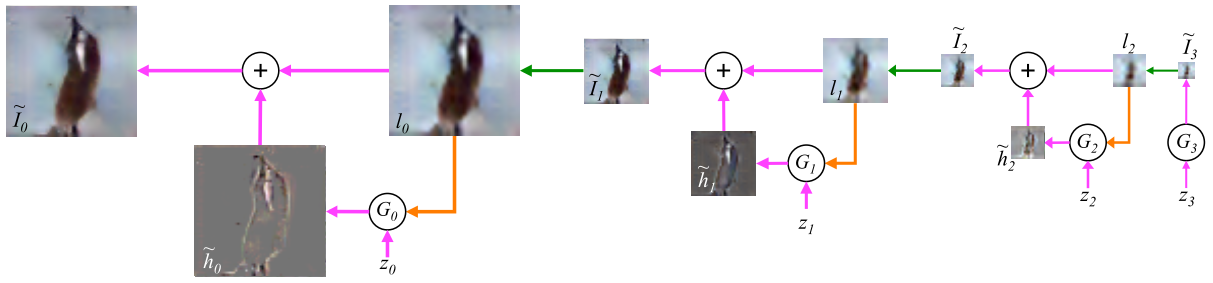
\includegraphics[width=0.9\linewidth]{img/lapgan_sampling}
	\caption{Sampling-Prozedur in LAPGANs (von rechts nach links)~\cite{Denton.2015}.}
	\label{fig:lapgansampling}
\end{figure}

Bis auf das erste \gls{gan} wird in diesem Fall auf jeder Ebene bereits eine konditionierte Variante der originalen \glspl{gan} verwendet.
Diese Modellvariante wurde schon bei \citeauthor{Goodfellow.2014}~\cite{Goodfellow.2014} vorgeschlagen und auch vor den LAPGANs bereits umgesetzt~\cite{Gauthier.2014,Mirza.2014}.
Im Kontext der konditionierten \glspl{gan} kommt eine konditionierende Variable $ \mathbf{y} $ hinzu, die sowohl an $ G $ als auch an $ D $ im Training und zur Inferenzzeit übergeben wird.
Dies erweitert die Zielfunktion von \autoref{eq:gan} zu

\begin{equation}
\begin{split}
\mathcal{L}_c(D, G) = & \ \mathbb{E}_{\mathbf{x}, \mathbf{y} \sim p_{\textup{data}}(\mathbf{x}, \mathbf{y})} [\log D(\mathbf{x}, \mathbf{y})] \\
+ & \ \mathbb{E}_{\mathbf{z} \sim p_{\mathbf{z}}(\mathbf{z}), \mathbf{y} \sim p_{\mathbf{y}}(\mathbf{y})} [\log(1 - D(G(\mathbf{z}, \mathbf{y}), \mathbf{y}))].
\end{split}
\end{equation}



\subsection{Deep Convolutional GANs}

Die \glspl{dcgan} von \citeauthor{Radford.2016}~\cite{Radford.2016} sind eine Weiterentwicklung der \glspl{gan}, deren Samples im Vergleich zu den LAPGANs weniger verrauscht sind.
Sie modifizieren die originalen \glspl{gan}, indem sie ähnlich den \glspl{fcn} nur noch Faltungsschichten statt Pooling- und vollständig verbundenen Schichten.
Außerdem nutzen sie in allen Schichten Batch-Normalisierung, was Mittelwert und Standardabweichung jedes Units einer Schicht auf respektive 0 und $ \pm 1 $ normiert.
Ebenso kommt als Aktivierungsfunktion im Generator nur noch das \gls{relu}~\cite{Nair.2010} und im Diskriminator das Leaky ReLU zum Einsatz; in der Ausgabeschicht des Generators erweist sich die Aktivierungsfunktion mit $ \tanh $ als erfolgreicher im Vergleich zu maxout bei den originalen \glspl{gan}.

Durch verschiedene Experimente können die Autoren zeigen, dass der latente Vektorraum, den das Modell lernt, tatsächlich glatte Übergänge hat, und dass die gelernten Filter zu häufig auftretenden Objekten korrespondieren.
Ebenso beobachten sie, dass das Unterdrücken von bestimmten Filtern dem Auslassen oder Transformieren bestimmter Objekte im generierten Sample entspricht, und dass simple Vektorarithmetik im latenten Vektorraum plausible Ergebnisse erzielt (s.~\autoref{fig:dcganarithmetic}).
All dies spricht dafür, dass diese Architektur nicht nur visuell ansprechende Ergebnisse erzielen kann, sondern auch eine stabile Repräsentation gelernt hat anstatt auswendig zu lernen und damit Overfitting zum Opfer zu fallen.

\begin{figure}
	\centering
	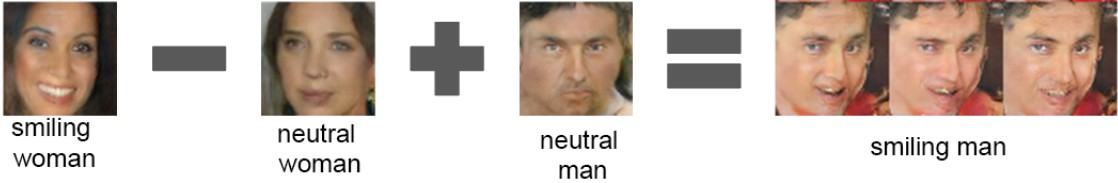
\includegraphics[width=0.9\linewidth]{img/dcgan_arithmetic}
	\caption{Beispiel für Vektorarithmetik in \glspl{dcgan}~\cite{Radford.2016}.}
	\label{fig:dcganarithmetic}
\end{figure}



\section{Conditional Adversarial Networks}

Die \glspl{can} von \citeauthor{Isola.2017}~\cite{Isola.2017} bestehen aus einem Generator und einem Diskriminator, die beide auf \glspl{dcgan} basieren.
Ihr Ansatz ist mit dem Zweck gestaltet, eine generische Architektur für Probleme bereitzustellen, bei denen eine Repräsentation eines Bildes auf eine andere Repräsentation eines Bildes abgebildet wird; die Autoren sprechen in diesem Zusammenhang von "Bild-zu-Bild-Übersetzung".
Im Gegensatz zu anderen Arbeiten, die konditionierte \glspl{gan} für spezielle Bild-zu-Bild-Probleme verwenden, ist in ihrer Architektur theoretisch \emph{nichts} anwendungsspezifisch angepasst.
Stattdessen ermöglicht es das GAN-Framework, dass die konkrete Verlustfunktion vollständig aus den Trainingsdaten gelernt wird, ohne dass diese problemspezifisch von Hand definiert werden muss.



\subsection{Generator}





\section{Form aus Sequenzbetrachtung}

Aus dem Stand der Technik und der Analyse von Koloskopie-Bildmaterial ergibt sich, dass neben sekundären Merkmalen wie Farbe und Textur die Form das aussagekräftigste Merkmal ist.
Aussagen über die Form würden wir am direktesten über die Tiefeninformation bekommen, aber wir haben oftmals nur monokulare Aufnahmen und damit keine unmittelbaren Tiefendaten vorliegen.
In der klassischen Bildverarbeitung ist es aber durch das Erfassen von Punktkorrespondenzen zwischen sequentiell aufgenommenen Bildern möglich, die Tiefeninformation einer Szene ungefähr zu rekonstruieren.
Dieser Bereich der Bildverarbeitung nennt sich "Structure from Motion".

Möglicherweise ist auch ein tiefes Netz dazu in der Lage, Tiefenstrukturen aus der Kamerabewegung abzuleiten.
Dazu muss man ihm allerdings mehrere konsekutive Frames zur Verfügung stellen.
Eine Architektur wie die 3D-FCNs liefert dafür eine gute Grundlage.

\subsection{3D-Faltung}

Den 3D-FCNs von \cite{Lequan.2017} liegen die 3D-CNNs zugrunde, welche zur Verarbeitung von dreidimensionalen Bilddaten genutzt werden können.
\citeauthor{Lequan.2017} nutzen diese allerdings unter der Annahme, dass ein Video auch nur ein 3D-Volumen ist.
Hierbei ist die zeitliche Komponente die dritte Dimension und die Zeitachse ihre Richtung -- es ergibt sich durch Aufeinanderstapeln der sequentiell angeordneten Frames ein 3D-Volumen.

[3D-Faltung erklären]

Bei den \glspl{can} ließe sich eine 3D-Faltung folgendermaßen umsetzen:
[]

\subsection{Optischer Fluss}

Zusätzlich zum 3D-Ansatz wäre auch eine reduzierte Variante mit optischem Fluss denkbar:
Man gibt dem Netz statt einem 3D-Volumen aus konsekutiven Frames einen einzelnen Frame inklusive der Information über den optischen Fluss vom vorherigen Frame zum jetzigen.
Je nach Geschwindigkeit des Tracking des optischen Flusses könnte dies die Gesamtperformanz des Systems theoretisch erhöhen, da maximal zwei Bilder auf einmal verarbeitet werden müssen.

Alle Teilansätze, die auf Seqenzbetrachtung beruhen, um Tiefeninformation zu generieren, sollten im Idealfall auch dann funktionieren, wenn nur ein einziger Input-Frame gegeben wird.

\subsection{Weitere DL-Methoden zur Tiefenschätzung}

\citeauthor{Mahmood.20171129} lassen mithilfe eines Transformer-GAN und Selbstregularisierung eine Transformation von realen zu synthetischen Bildern lernen, sodass dann auf dem synthetischen Bild die Tiefe geschätzt werden kann.
[sieht vielversprechend aus, aber steht uns nicht zur Verfügung]

\section{Dataset}

Im Zuge der MICCAI-Konferenz 2017 wurde auch eine neue Auflage der Endoscopic Vision Challenge ausgerichtet, die schon 2015 viele neue Ansätze in der endoskopischen Bildverarbeitung hervorbrachte.
Auch dieses Mal gab es wieder eine Sub-Challenge zur Polypen-Segmentierung, die Teil der GIANA ist.

[Herkunft der einzelnen Bestandteile des Datasets]

[Quantitative Beschreibung der Komponenten des Datasets]
